\newpage
\section*{Day 2 exercises}

In these exercises we transform a supply of $U \sim \mathcal{U}(0,1)$
variates from Day 1 into random variables $X$ with a prescribed distribution
function $F$, covering both discrete and continuous cases.
All simulations use $n = 10{,}000$ observations unless stated otherwise.

\section*{Exercise 2 --- Discrete Distributions}

% ================================================================
\section*{Part 1 --- Geometric Distribution}
% ================================================================

The Geometric($p$) distribution models the number of trials needed to get
the first success, where each trial succeeds independently with probability
$p$. The theoretical mean is $1/p$. As an example, if success has a 10\% chance, you
expect to need 10 trials on average.

We simulate $n = 10{,}000$ observations for three values of $p$ by inverting
$F(k) = 1-(1-p)^k$ (slide 9), giving
\begin{equation}
    X = \left\lfloor \frac{\log U}{\log(1-p)} \right\rfloor + 1.
    \label{eq:geom}
\end{equation}
and equivalently expressed in code as
\begin{verbatim}
return np.ceil(np.log(u) / np.log(1 - p)).astype(int)
\end{verbatim}
The sample mean is compared to the theoretical mean $1/p$, and a
chi-square goodness-of-fit test checks the simulated distribution against the
theoretical pmf, binning $k = 1, \ldots, k_{\max}$ and grouping the remaining
tail ($k > k_{\max}$) into one class, so $\mathrm{df} = k_{\max}$. Results are
in Table~\ref{tab:geom} and Figure~\ref{fig:geom}.

\begin{table}[h]
    \centering
    \caption{Geometric distribution results ($n = 10{,}000$).
             The sample mean is the average of the 10{,}000 simulated
             values; theory is the exact value $1/p$.}
    \label{tab:geom}
    \renewcommand{\arraystretch}{1.1}
    \begin{tabular}{lrrrr}
        \toprule
        $p$ & Sample mean & Theory ($1/p$) & $\chi^2$ & $p$-value \\
        \midrule
        $0.1$ & $10.01$ & $10.00$ & $43.22$ & $0.462$ \\
        $0.3$ & $3.39$  & $3.33$  & $19.50$ & $0.108$ \\
        $0.7$ & $1.41$  & $1.43$  & $27.53$ & $0.002$ \\
        \bottomrule
    \end{tabular}
\end{table}



The low $p$-value for $p = 0.7$ is a seed artefact: across 9 different seeds,
only seed 69 falls below $0.05$, which is consistent with the expected 5\%
false rejection rate under $H_0$.

Figure~\ref{fig:geom} shows the effect of $p$: small $p$ spreads the
distribution over many values (a rare success means many trials are needed),
while large $p$ concentrates almost all mass at $x = 1$.
 
\begin{figure}[h]
    \centering
    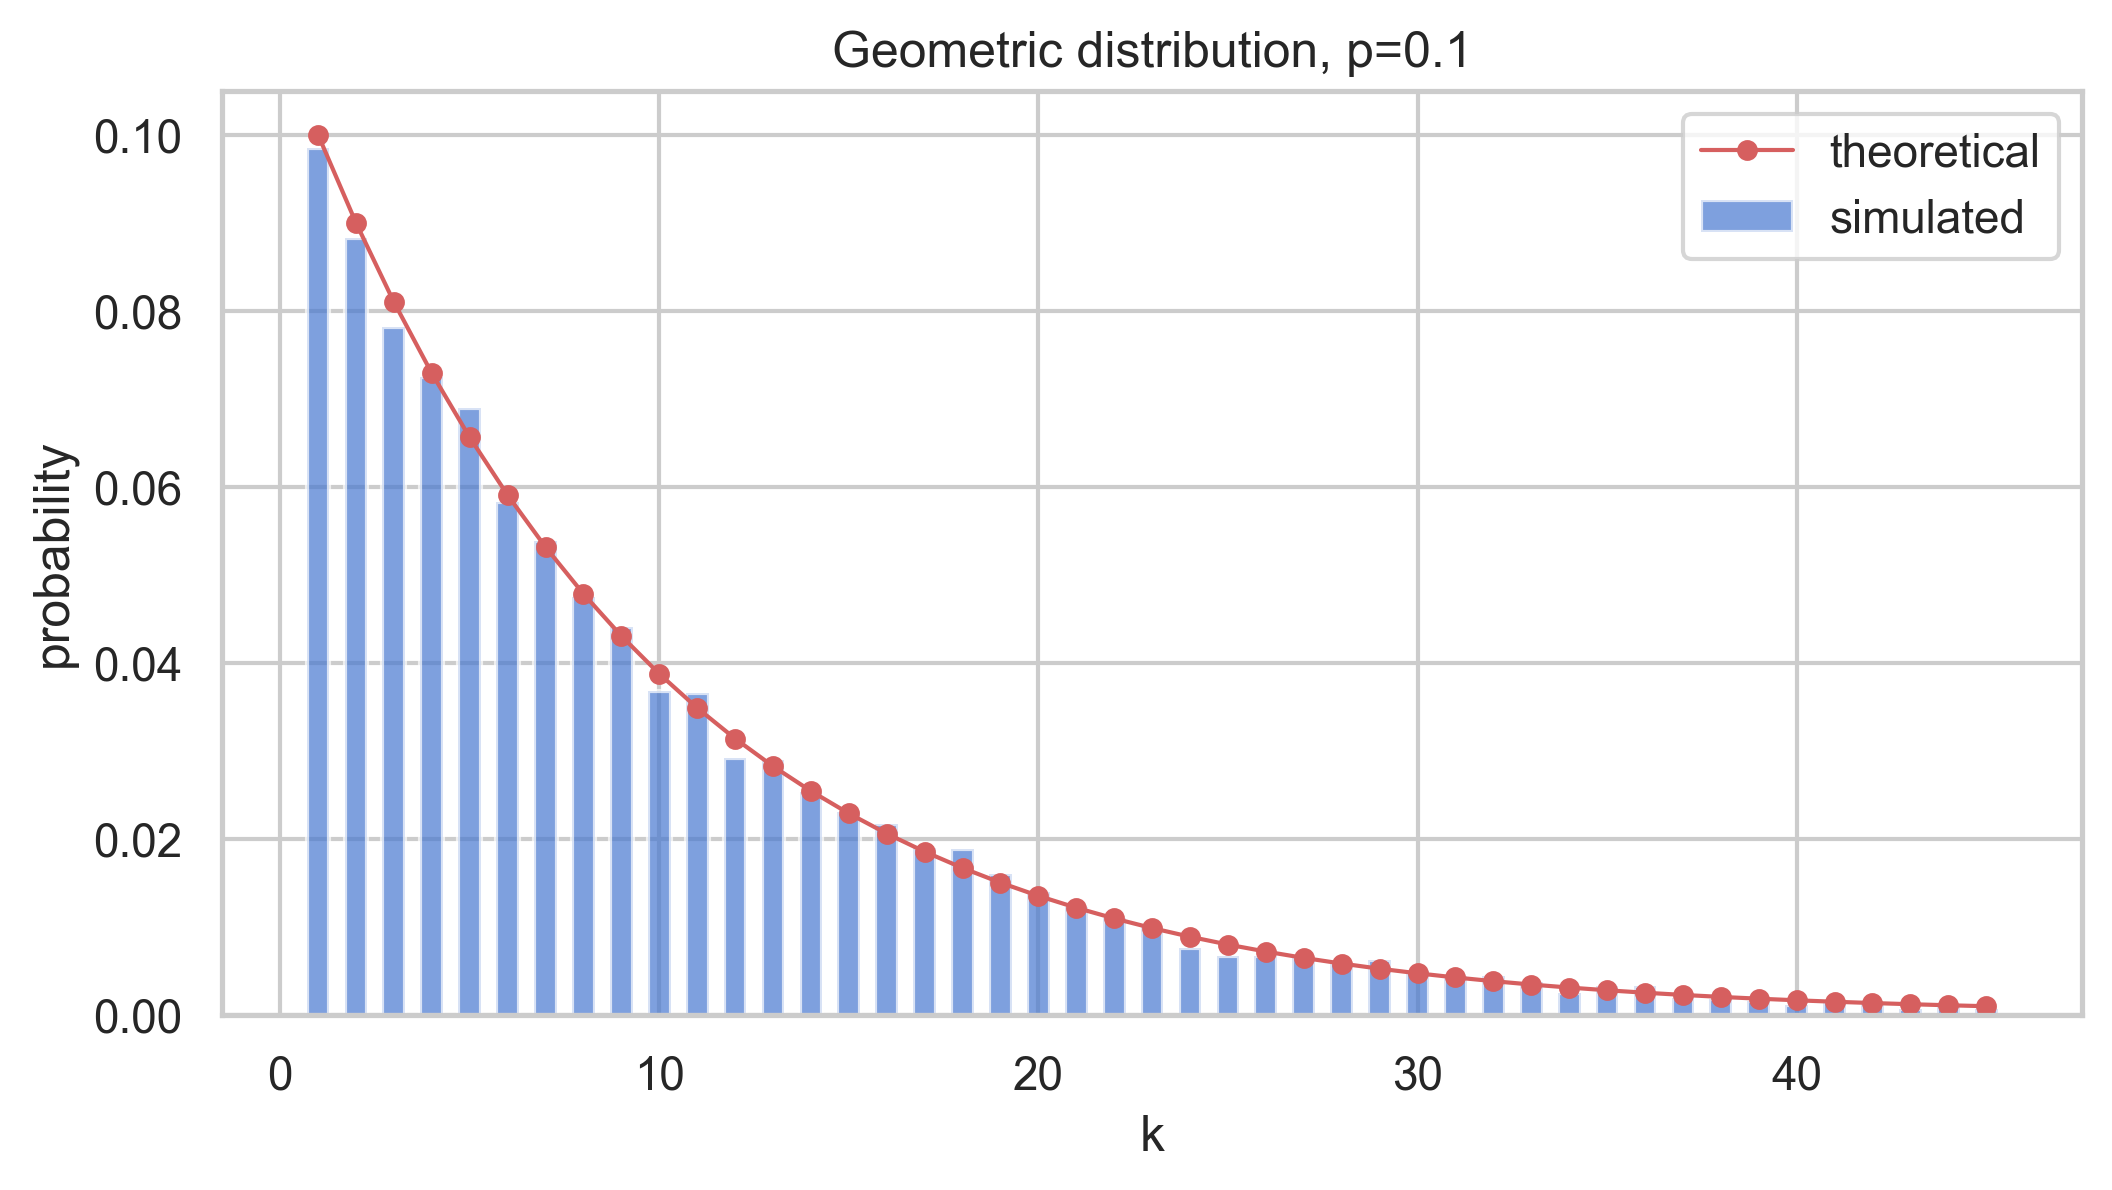
\includegraphics[width=0.32\textwidth]{plots/day2/geometric_p0.1.png}
    \hfill
    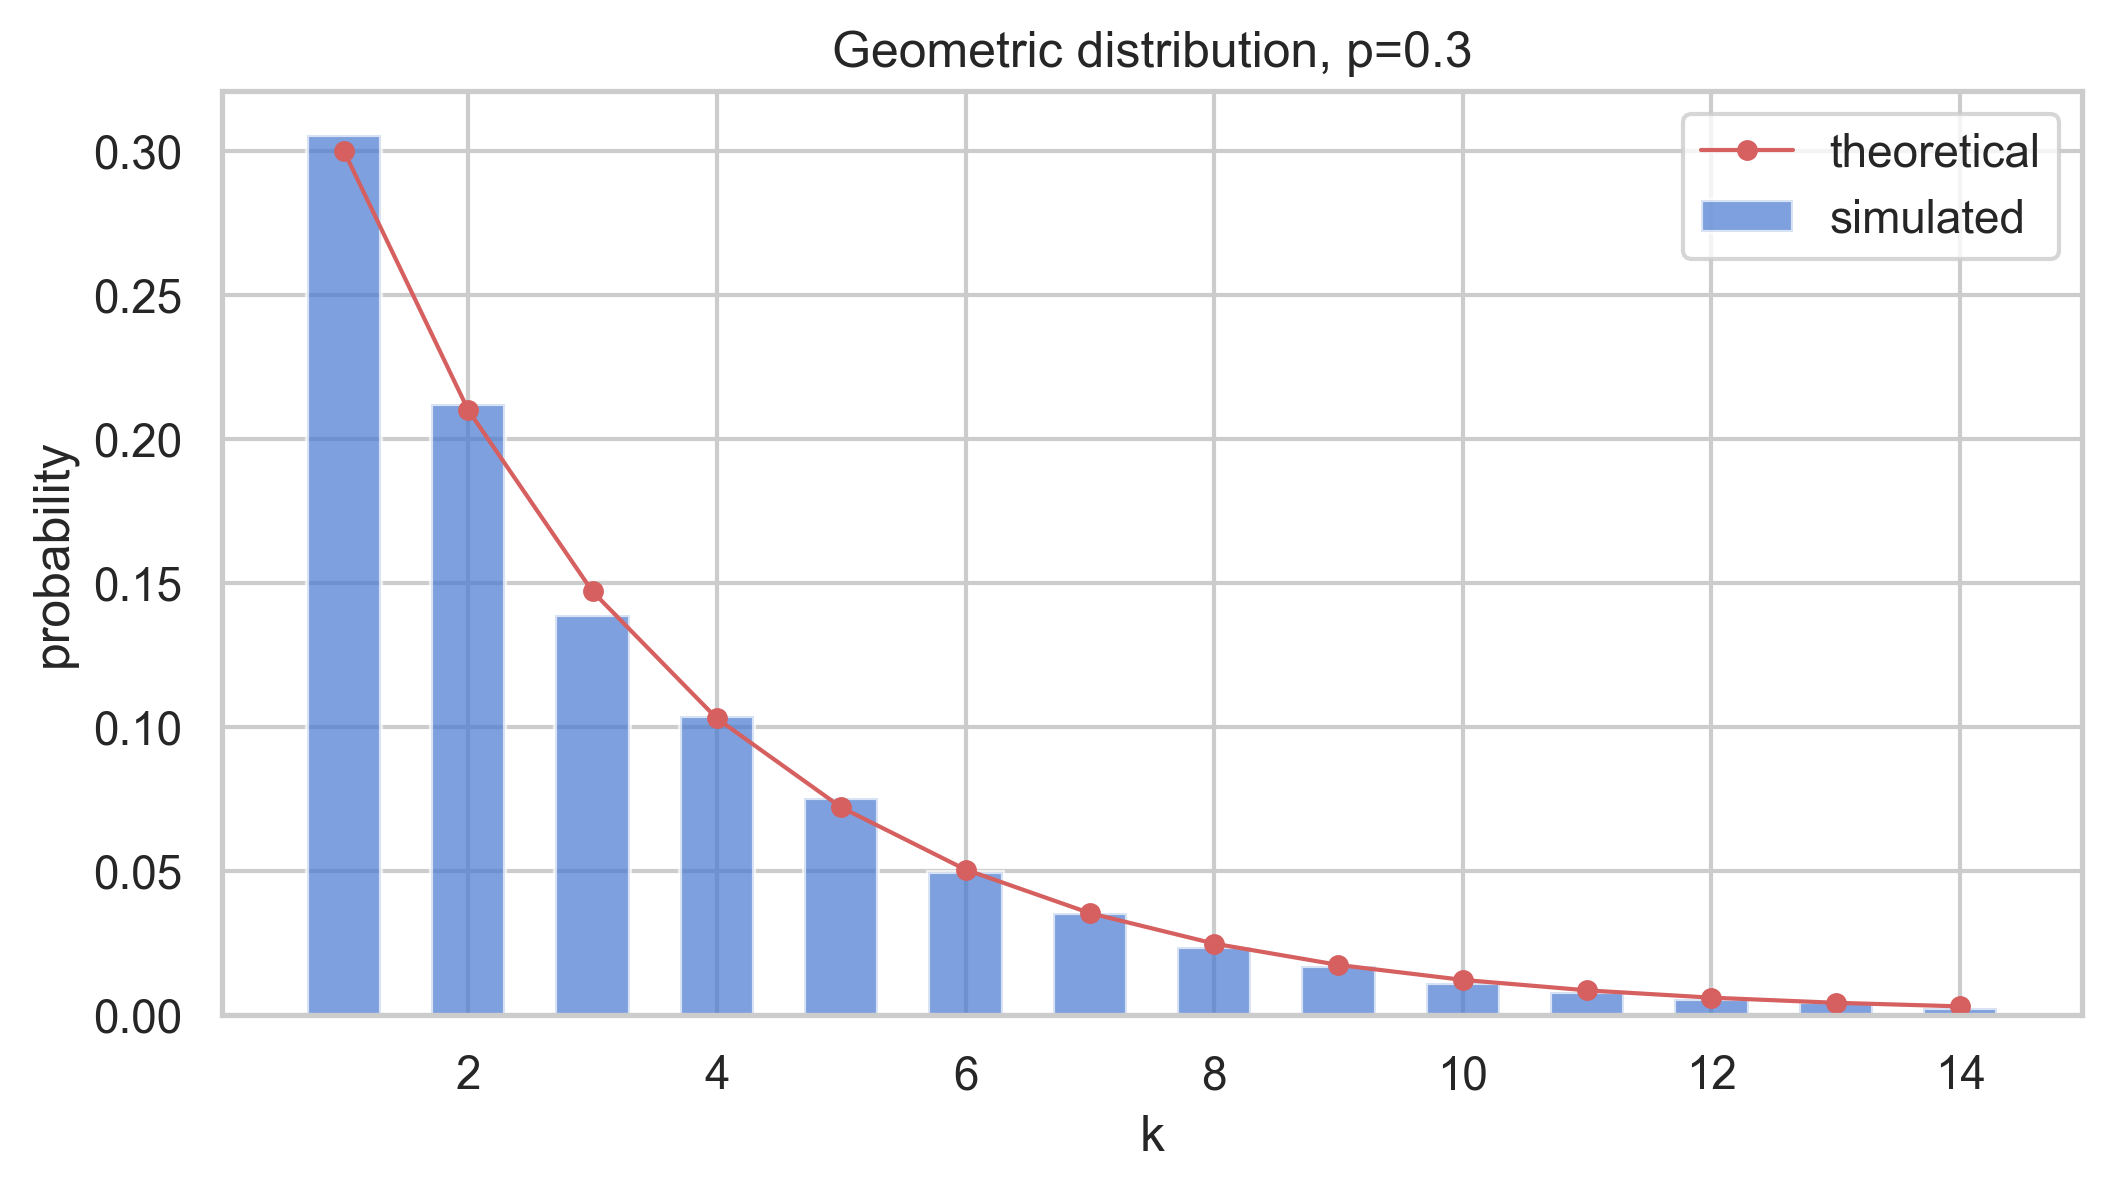
\includegraphics[width=0.32\textwidth]{plots/day2/geometric_p0.3.png}
    \hfill
    
\includegraphics[width=0.32\textwidth]{plots/day2/geometric_p0.7.png}
    \caption{Simulated (bars) vs.\ theoretical (dots) PMFs for
             $\text{Geometric}(p)$, $n = 10{,}000$.
             \textit{Left:} $p = 0.1$ --- heavy tail, spread over many values.
             \textit{Centre:} $p = 0.3$ --- moderate tail.
             \textit{Right:} $p = 0.7$ --- almost all mass at $x = 1$.}
    \label{fig:geom}
\end{figure}
 
% ================================================================
\section*{Part 2 --- Six-Point Distribution}
% ================================================================
 
The six-point distribution is a made-up discrete distribution with six
outcomes $\{1, 2, 3, 4, 5, 6\}$ and unequal probabilities --- unlike a
fair die. Outcome 6 is the most likely ($\approx 31\%$) and outcome 4 is
the least likely ($\approx 6\%$):
\begin{center}
\renewcommand{\arraystretch}{1.1}
\begin{tabular}{lrrrrrr}
    \toprule
    $x_i$               & 1              & 2              & 3             & 4              & 5             & 6              \\
    \midrule
    $\mathbb{P}(X=x_i)$ & $\tfrac{7}{48}$ & $\tfrac{5}{48}$ & $\tfrac{1}{8}$ & $\tfrac{1}{16}$ & $\tfrac{1}{4}$ & $\tfrac{5}{16}$ \\
    \bottomrule
\end{tabular}
\end{center}
 
Three sampling methods are implemented and applied to this pmf, each with
$k = 6$ outcomes:

\textbf{Crude/direct inversion} returns $X = x_i$ whenever
$F(x_{i-1}) < U \leq F(x_i)$ (slide 8), i.e.\ a binary
search of $U$ into the cumulative table (\texttt{crude\_sample}, using
\texttt{np.searchsorted}):
\begin{verbatim}
return np.searchsorted(cdf, u, side="left") + 1
\end{verbatim}

\textbf{Simple rejection} proposes $I = \lfloor kU_1 \rfloor + 1$ and accepts
it if $U_2 \leq p_I / c$ with $c = \max_i p_i$ (slide 11,
correctness proved on slide 18). Here $c = 5/16$ and $k = 6$:
\begin{verbatim}
accepted = idx[u <= probs[idx] / c]
\end{verbatim}

\textbf{Alias method} builds probability and alias tables $(F, L)$ once, then
draws $I = \lfloor kU_1 \rfloor + 1$ and returns $I$ if $U_2 \leq F(I)$, else
$L(I)$ (slides 14--16). The draw is one comparison, but the setup is the
real work, where it partitions the scaled probabilities into deficient
($<1$) and surplus ($\geq 1$) columns and pairs them off (slide 12):
\begin{verbatim}
prob = n * probs                  # column heights, mean 1
small = [i for i in range(n) if prob[i] < 1.0]
large = [i for i in range(n) if prob[i] >= 1.0]
while small and large:
    l = small.pop()
    g = large[-1]
    alias[l] = g                  # g fills the rest of l's column
    prob[g] += prob[l] - 1.0
    if prob[g] < 1.0:
        large.pop()
        small.append(g)
\end{verbatim}

The chi-square goodness-of-fit test has 6 classes, so $\mathrm{df} = 5$. We
run each method with two seeds to show that the $p$-value itself is random.

\begin{table}[h]
    \centering
    \caption{Chi-square results for the six-point distribution,
             $n = 10{,}000$. $H_0$ is rejected if $p < 0.05$.}
    \label{tab:sixpoint}
    \renewcommand{\arraystretch}{1.1}
    \begin{tabular}{lrrrr}
        \toprule
        & \multicolumn{2}{c}{Seed 42} & \multicolumn{2}{c}{Seed 69} \\
        \cmidrule(lr){2-3} \cmidrule(lr){4-5}
        Method    & $\chi^2$ & $p$-value & $\chi^2$ & $p$-value \\
        \midrule
        Crude     & $2.96$ & $0.706$ & $3.57$ & $0.613$ \\
        Rejection & $3.77$ & $0.583$ & $7.39$ & $0.193$ \\
        Alias     & $2.94$ & $0.709$ & $7.34$ & $0.196$ \\
        \bottomrule
    \end{tabular}
\end{table}

All six $p$-values exceed 0.05, but they differ noticeably between seeds for
the same sampler --- the $p$-value is itself a random draw from
$\mathcal{U}(0,1)$ under $H_0$, so some scatter is expected even when every
method is correct.

\begin{figure}[h]
    \centering
    
\includegraphics[width=0.32\textwidth]{plots/day2/sixpoint_crude.png}
    \hfill
    
\includegraphics[width=0.32\textwidth]{plots/day2/sixpoint_rejection.png}
    \hfill
    
\includegraphics[width=0.32\textwidth]{plots/day2/sixpoint_alias.png}
    \caption{Simulated (blue bars) vs.\ theoretical (orange bars) PMFs for the six-point
             distribution, seed 69, $n = 10{,}000$.
             \textit{Left:} Crude.
             \textit{Centre:} Rejection.
             \textit{Right:} Alias.}
    \label{fig:sixpoint}
\end{figure}
 
% ================================================================
\section*{Part 3 --- Method Comparison}
% ================================================================

Since all three methods are correct (verified in Part 2 via chi-squared tests), we focus on how efficiently they generate samples. With $n = 10{,}000$, the timings are dominated by noise and random variation; we therefore use $n = 1{,}000{,}000$ for a reliable comparison. Table~\ref{tab:comparison} summarises the key performance measures.

\begin{table}[h]
\centering
\caption{Performance comparison of the three generation methods at $n = 1{,}000{,}000$, seed 69.}
\label{tab:comparison}
\renewcommand{\arraystretch}{1.2}
\begin{tabular}{lrrrcc}
\toprule
Method    & $\chi^2$ & $p$-value & Time (s) & Uniforms per draw & Work per draw \\
\midrule
Crude     & 3.39     & 0.640     & 0.021    & 1                 & $O(\log k)$ \\
Rejection & 2.66     & 0.753     & 0.030    & $\approx 3.75$    & $O(1)$ per proposal \\
Alias     & 3.15     & 0.677     & 0.016    & 2                 & $O(1)$ \\
\bottomrule
\end{tabular}
\end{table}

All three methods pass the goodness-of-fit test ($p \gg 0.05$), so accuracy is not a differentiator. The alias method is fastest, requiring exactly two uniforms and $O(1)$ work per draw regardless of $k$. The crude method needs only one uniform but pays $O(\log k)$ per draw for the binary search over the CDF. The rejection method is slowest: using a discrete uniform proposal gives an acceptance probability of $1/(k \max_i p_i) = 1/(6 \cdot 5/16) \approx 0.53$, so on average $\approx 1.88$ proposals and $\approx 3.75$ uniforms are consumed per accepted sample. All three methods share $O(k)$ memory; the alias method additionally requires an $O(k)$ precomputation step to build its two lookup tables. The work-per-draw complexities are standard results looked up online rather than derived here.

\section*{Part 4 — Recommendations}

For a fixed pmf sampled many times, we recommend the alias method: it achieves $O(1)$ per draw regardless of $k$ or pmf shape, at the cost of a one-time $O(k)$ setup. When the pmf changes between draws or $k$ is small, we recommend the crude method, as it requires no setup and only one uniform per sample. We would only recommend the rejection method when the pmf is near-uniform or unnormalised (e.g.\ in MCMC), since its acceptance rate $1/(k\max_i p_i)$ degrades rapidly for peaked distributions — for this six-point pmf it already wastes nearly half its proposals. See Table~\ref{tab:recommendations} for an overview.

\begin{table}[h]
\centering
\caption{Overview of recommendations for each generation method.}
\label{tab:recommendations}
\renewcommand{\arraystretch}{1.2}
\begin{tabular}{lp{4.2cm}p{6cm}}
\toprule
Method    & Prefer when & Avoid when \\
\midrule
Crude     & Small $k$, changing pmf, or quick prototyping  & Large $k$ with many draws \\
Alias     & Fixed pmf, large $k$ or large $n$              & pmf changes frequently \\
Rejection & Near-uniform pmf or unnormalised distributions & Peaked pmf over large $k$ \\
\bottomrule
\end{tabular}
\end{table}

\newpage 
% ================================================================
\section*{Exercise 3 --- Continuous Distributions}
% ================================================================

We implement inverse-transform and Box--Muller samplers for three continuous
distributions and verify them via Kolmogorov--Smirnov (KS) tests, using the
principle that $Y = F_X^{-1}(U) \sim F_X$ for $U \sim \mathcal{U}(0,1)$
(slide 5). All
samples use $n = 10{,}000$.

% ================================================================
\section*{Part 1 --- Sampling and KS Tests}
% ================================================================

\textbf{Exponential.} Inverting $F(x) = 1 - e^{-\lambda x}$ gives
\begin{equation}
    X = -\frac{\log U}{\lambda}
    \label{eq:exp}
\end{equation}
(slide 6):
\begin{verbatim}
return -np.log(u) / lam
\end{verbatim}

\textbf{Pareto Type I.} For $F(x) = 1 - (\beta/x)^k$, $x \geq \beta$, with
$E[X] = \beta k/(k-1)$ and $V[X] = \beta^2 k / ((k-1)^2(k-2))$, inversion gives
\begin{equation}
    X = \beta U^{-1/k}
    \label{eq:pareto}
\end{equation}
(slide 7):
\begin{verbatim}
return beta / u ** (1.0 / k)
\end{verbatim}

\textbf{Normal (Box--Muller).} Two independent uniforms map to two
independent $N(0,1)$ variates via the Rayleigh-distributed radius
$R = \sqrt{-2\log U_1}$ and angle $\Theta = 2\pi U_2$:
\begin{equation}
    (Z_1, Z_2) = \big(\sqrt{-2\log U_1}\cos(2\pi U_2),\ \sqrt{-2\log U_1}\sin(2\pi U_2)\big)
    \label{eq:boxmuller}
\end{equation}
(slides 9 and 11):
\begin{verbatim}
r = np.sqrt(-2.0 * np.log(u1))
theta = 2.0 * np.pi * u2
z = np.concatenate([r * np.cos(theta), r * np.sin(theta)])
\end{verbatim}

Each sample is verified with a one-sample Kolmogorov--Smirnov (KS) test, which measures $D = \sup_x |F_n(x) - F(x)|$ --- the maximum gap between the empirical and theoretical CDFs --- without requiring any binning. The $\chi^2$ test from Exercise 2 is not used here: for continuous data, bin choices are arbitrary and degrade power, particularly in the tails. Results are in Table~\ref{tab:ks} and Figure~\ref{fig:continuous}.

\begin{table}[h]
    \centering
    \caption{KS goodness-of-fit results ($n = 10{,}000$). Sample mean is
             compared to the theoretical mean.}
    \label{tab:ks}
    \renewcommand{\arraystretch}{1.1}
    \begin{tabular}{lrrrr}
        \toprule
        Distribution & Sample mean & Theory & KS stat & $p$-value \\
        \midrule
        Exponential ($\lambda=1$) & $1.0062$ & $1.0000$ & $0.0074$ & $0.634$ \\
        Normal (Box--Muller)      & $0.0007$ & $0.0000$ & $0.0054$ & $0.928$ \\
        Pareto $k=2.05$           & $1.9723$ & $1.9524$ & $0.0082$ & $0.503$ \\
        Pareto $k=2.5$            & $1.6650$ & $1.6667$ & $0.0080$ & $0.546$ \\
        Pareto $k=3.0$            & $1.4977$ & $1.5000$ & $0.0057$ & $0.904$ \\
        Pareto $k=4.0$            & $1.3371$ & $1.3333$ & $0.0052$ & $0.949$ \\
        \bottomrule
    \end{tabular}
\end{table}

All $p$-values are well above $0.05$: every sampler reproduces its target
distribution, and the histograms in Figure~\ref{fig:continuous} track the
analytical pdfs closely, including in the heavy tail of the small-$k$ Pareto
cases.

\begin{figure}[h]
    \centering
    
\includegraphics[width=0.32\textwidth]{plots/day2/exponential.png}
    \hfill
    
\includegraphics[width=0.32\textwidth]{plots/day2/normal.png}
    \hfill
    
\includegraphics[width=0.32\textwidth]{plots/day2/pareto_all.png}
    \caption{Simulated histograms (bars) vs.\ analytical pdfs (red), $n = 10{,}000$.
             \textit{Left:} Exponential($\lambda=1$).
             \textit{Centre:} Normal via Box--Muller.
             \textit{Right:} Pareto($\beta=1$) for $k \in \{2.05, 2.5, 3, 4\}$.}
    \label{fig:continuous}
\end{figure}

% ================================================================
\section*{Part 2 --- Pareto Moments}
% ================================================================

For $\text{Pareto}(\beta, k)$, the theoretical mean and variance are
$E[X] = \beta k/(k-1)$ and $V[X] = \beta^2 k / ((k-1)^2(k-2))$ (slide 7),
defined only for
$k > 1$ and $k > 2$ respectively. Table~\ref{tab:moments} compares these to
the sample moments from the $n = 10{,}000$ draws of Part 1.

\begin{table}[h]
    \centering
    \caption{Sample vs.\ theoretical moments for Pareto($\beta=1$), $n = 10{,}000$.}
    \label{tab:moments}
    \renewcommand{\arraystretch}{1.1}
    \begin{tabular}{lrrrr}
        \toprule
        $k$ & $E[X]$ sim & $E[X]$ theory & $V[X]$ sim & $V[X]$ theory \\
        \midrule
        $2.05$ & $1.9452$ & $1.9524$ & $9.96$  & $37.19$ \\
        $2.5$  & $1.6479$ & $1.6667$ & $1.44$  & $2.22$  \\
        $3.0$  & $1.5042$ & $1.5000$ & $0.68$  & $0.75$  \\
        $4.0$  & $1.3373$ & $1.3333$ & $0.22$  & $0.22$  \\
        \bottomrule
    \end{tabular}
\end{table}

The means agree well for all $k$, but the variance at $k = 2.05$, we see a big difference: with $k - 2 = 0.05$ the denominator $(k-1)^2(k-2)$ is tiny, so
$V[X] \approx 37.19$ is very large compared to the sample value of $9.96$. The
variance of a Pareto with $k$ close to 2 is dominated by extremely rare,
extremely large draws from its heavy power-law tail; $n = 10{,}000$ samples
essentially never see them, so the sample variance severely underestimates
the true value. We verified this across 12 different seeds: sample variances
ranged from $3.8$ to $13.6$, never approaching the theoretical $37.19$, and
the spread itself reflects how much a single large draw can shift the estimate ---
seed 500 drew a maximum of $221$, giving the highest sample variance of $13.6$,
while most seeds topped out around $50$--$140$ and yielded variances of $4$--$7$.
To reliably estimate a variance this large would require $n$ in the millions.
For $k \leq 2$, $V[X]$ is theoretically infinite and no finite
sample can estimate it consistently. This motivates variance reduction
techniques covered in later exercises, which improve estimation efficiency
precisely in situations where the naive Monte Carlo estimator has high variance.

% ================================================================
\section*{Part 3 --- Normal Confidence Intervals}
% ================================================================

Using the $N(0,1)$ sampler from Part 1, we draw 100 independent samples of
$n = 10$ and construct a 95\% CI for the mean and for the variance from each.

The mean CI uses the Student-$t$ pivot rather than the normal, because $\sigma^2$
is unknown and must be estimated by $s^2$. Replacing $\sigma$ with $s$ makes the
pivot heavier-tailed than the normal --- that extra uncertainty is exactly what
the $t$-distribution accounts for:
\begin{equation}
    \bar{x} \pm t_{0.975,\,9}\sqrt{s^2/n}.
    \label{eq:ci-mean}
\end{equation}

The variance CI uses the $\chi^2$ pivot. Because the $\chi^2$ distribution is
right-skewed, the two quantile cuts are not symmetric: $\chi^2_{0.025,9} \approx 2.70$
whereas $\chi^2_{0.975,9} \approx 19.02$, so the interval is wider on the left
than on the right:
\begin{equation}
    \left(\frac{(n-1)s^2}{\chi^2_{0.975,\,9}},\ \frac{(n-1)s^2}{\chi^2_{0.025,\,9}}\right).
    \label{eq:ci-var}
\end{equation}

Coverage is the fraction of the 100 intervals that contain the true value
($\mu = 0$, $\sigma^2 = 1$).

\begin{table}[h]
    \centering
    \caption{Coverage of $100 \times 95\%$ confidence intervals from $n=10$ samples.}
    \label{tab:ci}
    \renewcommand{\arraystretch}{1.1}
    \begin{tabular}{lrr}
        \toprule
        CI for & Coverage & Expected \\
        \midrule
        Mean     & $94/100$ & $\approx 95$ \\
        Variance & $96/100$ & $\approx 95$ \\
        \bottomrule
    \end{tabular}
\end{table}

Both coverages are consistent with the nominal 95\% level: the binomial
standard error of a count out of 100 at $p=0.95$ is $\approx 2.2$, so $94$
and $96$ are both within one standard error of $95$. With only $n=10$
observations the intervals are wide --- with $t_{0.975,9} \approx 2.26$ and
$s \approx 1$, a typical half-width is $2.26/\sqrt{10} \approx 0.71$, so each
interval spans roughly $\pm 0.71$ around the sample mean. The red intervals
in Figure~\ref{fig:ci} are the ones that miss $\mu=0$.

\begin{figure}[h]
    \centering
    
\includegraphics[width=0.6\textwidth]{plots/day2/ci_mean.png}
    \caption{$100 \times 95\%$ confidence intervals for the mean, $n=10$ draws
             from the Box--Muller $N(0,1)$ sampler of Part 1. Blue intervals
             contain $\mu=0$; red intervals do not. Coverage shown in Table~\ref{tab:ci}.}
    \label{fig:ci}
\end{figure}

% ===============================================================
\section*{Part 4 --- Pareto via Composition}
% ===============================================================

Instead of generating Pareto samples directly with the inversion formula from
Part 1, the composition method breaks it into two simpler steps:
\begin{enumerate}
    \item Draw a random rate $\Lambda \sim \text{Gamma}(\text{shape}=k,\ \text{scale}=1/\beta)$.
    \item Draw $X = \beta + Y$ where $Y \sim \text{Exponential with rate } \Lambda$
          (i.e.\ mean $1/\Lambda$).
\end{enumerate}

\begin{verbatim}
lam = rng.gamma(shape=k, scale=1.0 / beta)
return beta + rng.exponential(scale=1.0 / lam)
\end{verbatim}

The result is Pareto-distributed, even though the Pareto formula was never
used directly. This works because the Pareto distribution can be written as a
mixture of exponentials with a Gamma-distributed rate: if you integrate
$\Lambda$ out of the joint density, you recover $f_X(x) = k\beta^k / x^{k+1}$,
which is exactly the Pareto pdf.

For $k = 3$, $\beta = 1$, we check that this produces the same distribution
as the inversion method from Part 1. Two KS tests confirm this: one compares
the composition samples to the theoretical Pareto pdf, the other compares
them directly to the inversion samples from Part 1. Both pass comfortably
(Table~\ref{tab:composition}).

\begin{table}[h]
    \centering
    \caption{KS tests for the composition sampler ($k = 3$, $\beta = 1$,
             $n = 10{,}000$). Both $p$-values are far above 0.05.}
    \label{tab:composition}
    \renewcommand{\arraystretch}{1.1}
    \begin{tabular}{lrr}
        \toprule
        Comparison                          & KS stat & $p$-value \\
        \midrule
        Composition vs.\ theoretical Pareto & $0.0060$ & $0.860$ \\
        Composition vs.\ inversion samples  & $0.0109$ & $0.592$ \\
        \bottomrule
    \end{tabular}
\end{table}

Both methods produce the same distribution. For Pareto, inversion is simpler
since there is a nice closed-form formula. The composition method is useful
when no such formula exists and you need to break the distribution into
simpler pieces.